\section{Finding optimal bandwidth}
\subsection{}
If $x\in B_j$, then
\begin{align*}
	\hat{f}(x) & = \frac{\textrm{number of observations within }B_j}{n} \times \frac{1}{\textrm{length of the bin}} \\
	           & =  \frac{v_j}{n} \times \frac{1}{h}
\end{align*}
Since $x$ belongs to exactly one $B_j$, we can write
\begin{align*}
	\hat{f}(x)   & = \sum_{j=1}^m \frac{v_j}{nh} I\left(x\in B_j\right)                                                                                                 \\
	\hat{f}(x)^2 & = \frac{1}{n^2h^2} \left(\sum_{j=1}^m I\left(x\in B_j\right) v_j \right)^2                                                                           \\
	             & = \frac{1}{n^2h^2} \left(\sum_{j=1}^m I\left(x\in B_j\right)^2 v_j^2 + 2\sum_{1\leq i < j \leq m} I\left(x \in B_i\right)I(x \in B_j)v_i v_j \right)
\end{align*}
Again, since $x$ belongs to exactly one $B_j$, i.e., $I\left(x\in B_j\right)$ for exactly one $j$. Thus, we can say that $I(x\in B_i) I\left(x\in B_j\right) = 0$ for distinct $i$ and $j$.
Also, $I\left(x\in B_j\right)^2 = I\left(x\in B_j\right)$, as $I\left(x\in B_j\right)$ is either 0 or 1. Thus, we can write
\begin{align*}
	\hat{f}(x)^2         & = \frac{1}{n^2h^2} \sum_{j=1}^m I\left(x\in B_j\right) v_j^2         \\
	\int \hat{f}(x)^2 dx & = \frac{1}{n^2h^2} \sum_{j=1}^m v_j^2 \int I\left(x\in B_j\right) dx
\end{align*}
$I\left(x\in B_j\right)$ is one, only over $B_j$. So, the integral is the length of $B_j$, i.e., $h$. Thus, we can write
\begin{align*}
	\int \hat{f}(x)^2 dx            & = \frac{1}{n^2h^2} \sum_{j=1}^m v_j^2 h \\
	\therefore \int \hat{f}(x)^2 dx & = \frac{1}{n^2h} \sum_{j=1}^m v_j^2
\end{align*}
\subsection{}
\subsubsection*{(a)}
\vspace{-30pt}
\begin{figure}[H]
	\centering
	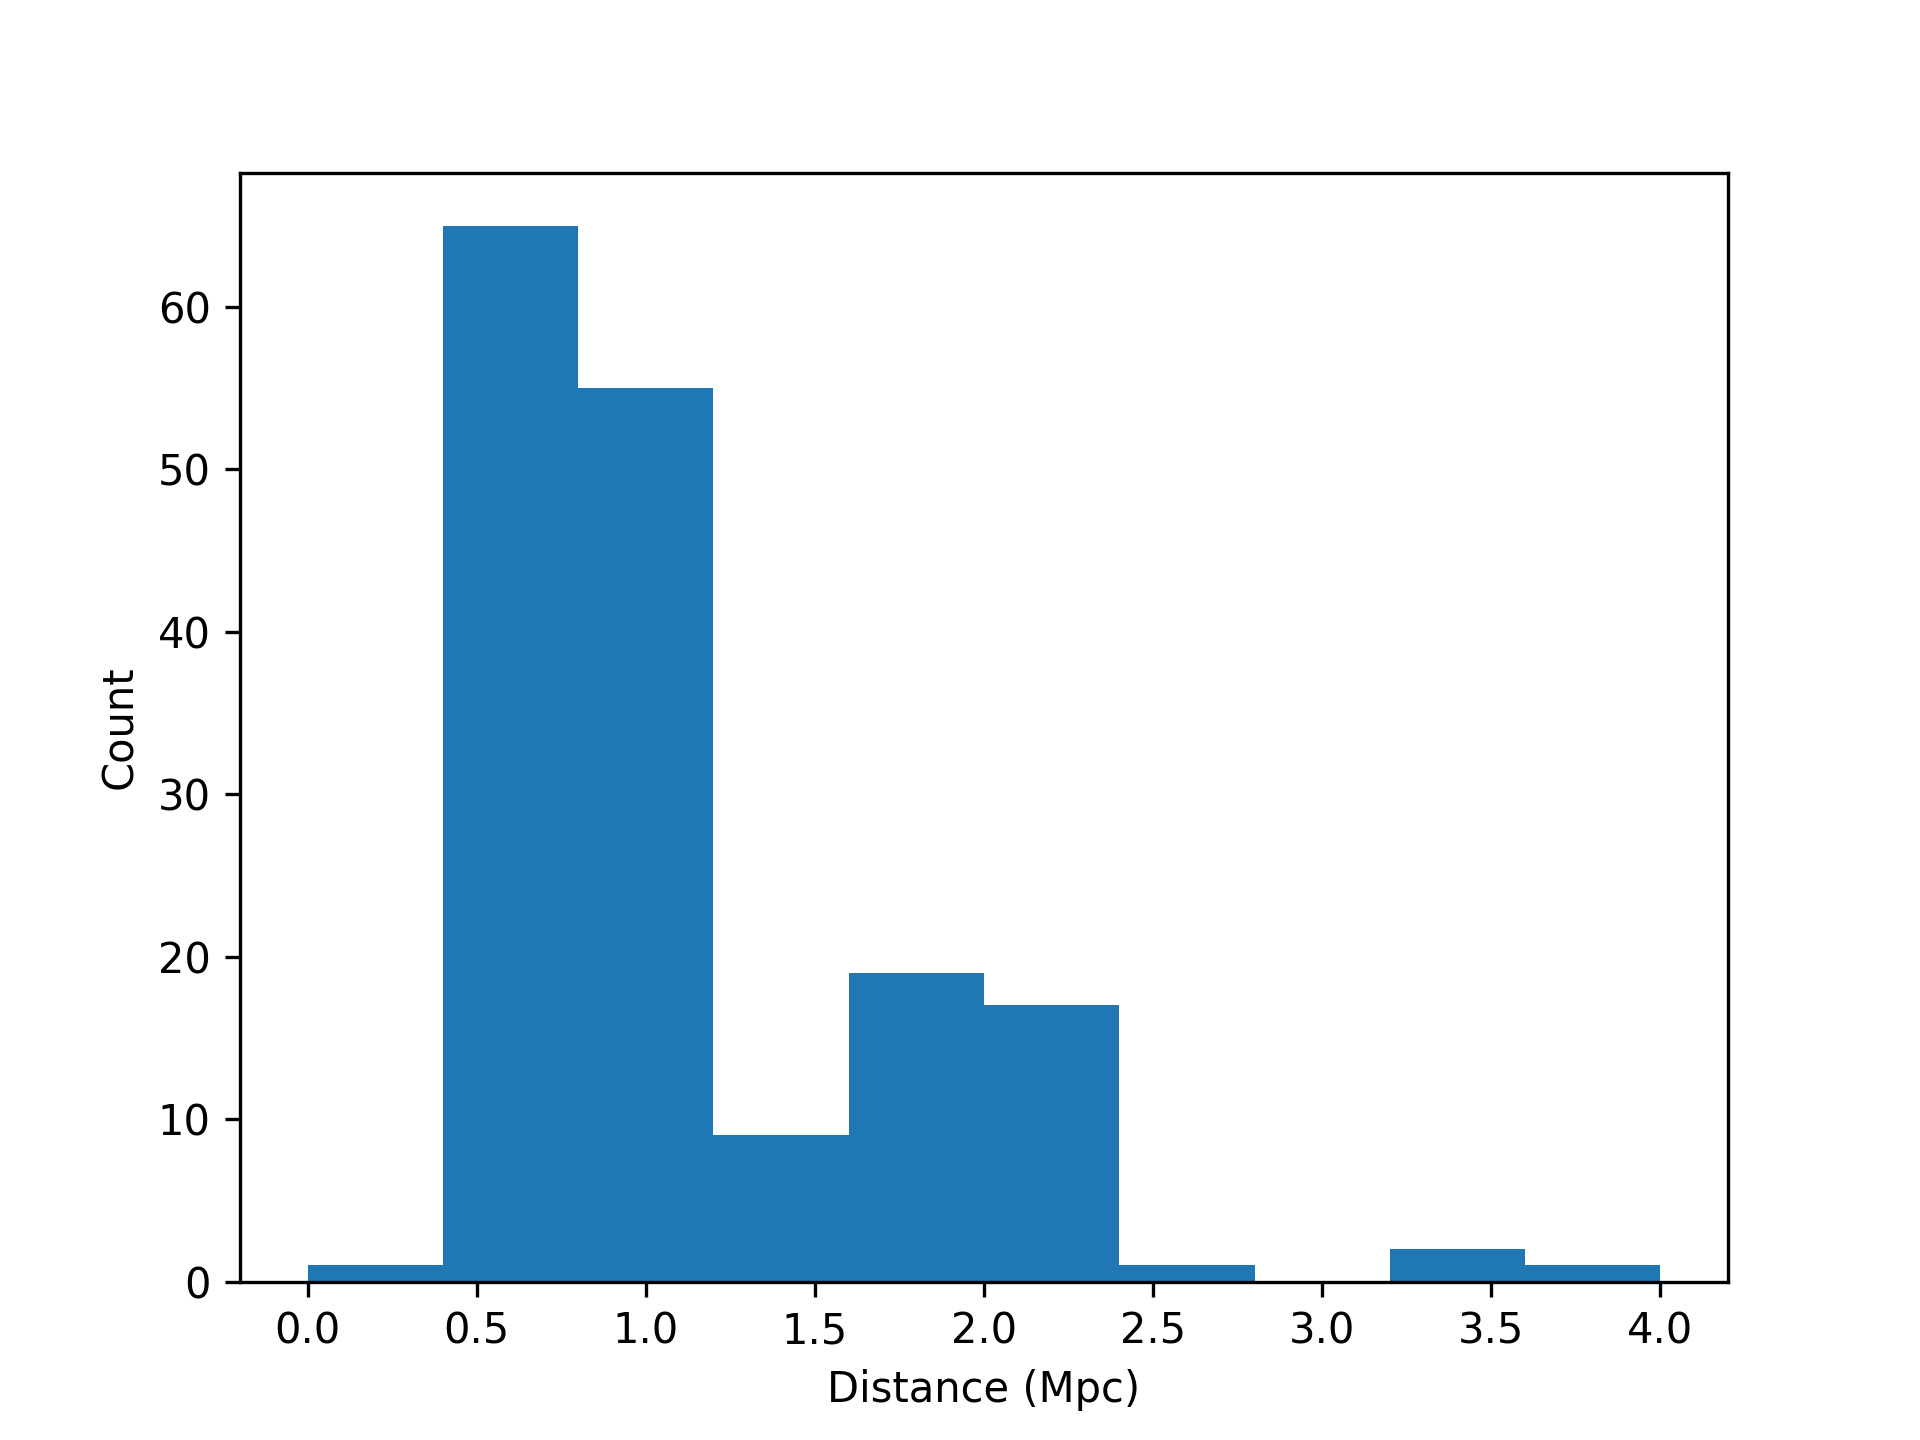
\includegraphics[width=0.6\textwidth]{images/1/10binhistogram.png}
	\caption{Histogram with 10 bins}
\end{figure}
The estimated probabilities for the bins are\\
\texttt{[0.00588235 0.38235294 0.32352941 0.05294118 0.11176471 0.1
			0.00588235 0.         0.01176471 0.00588235]}

\subsubsection*{(b)}
The probability distribution is oversmoothed, as the histogram has too few bins to capture the distribution of the data. It does not capture the rough peaks of the actual distribution.

\subsubsection*{(c)}
\vspace{-30pt}
\begin{figure}[H]
	\centering
	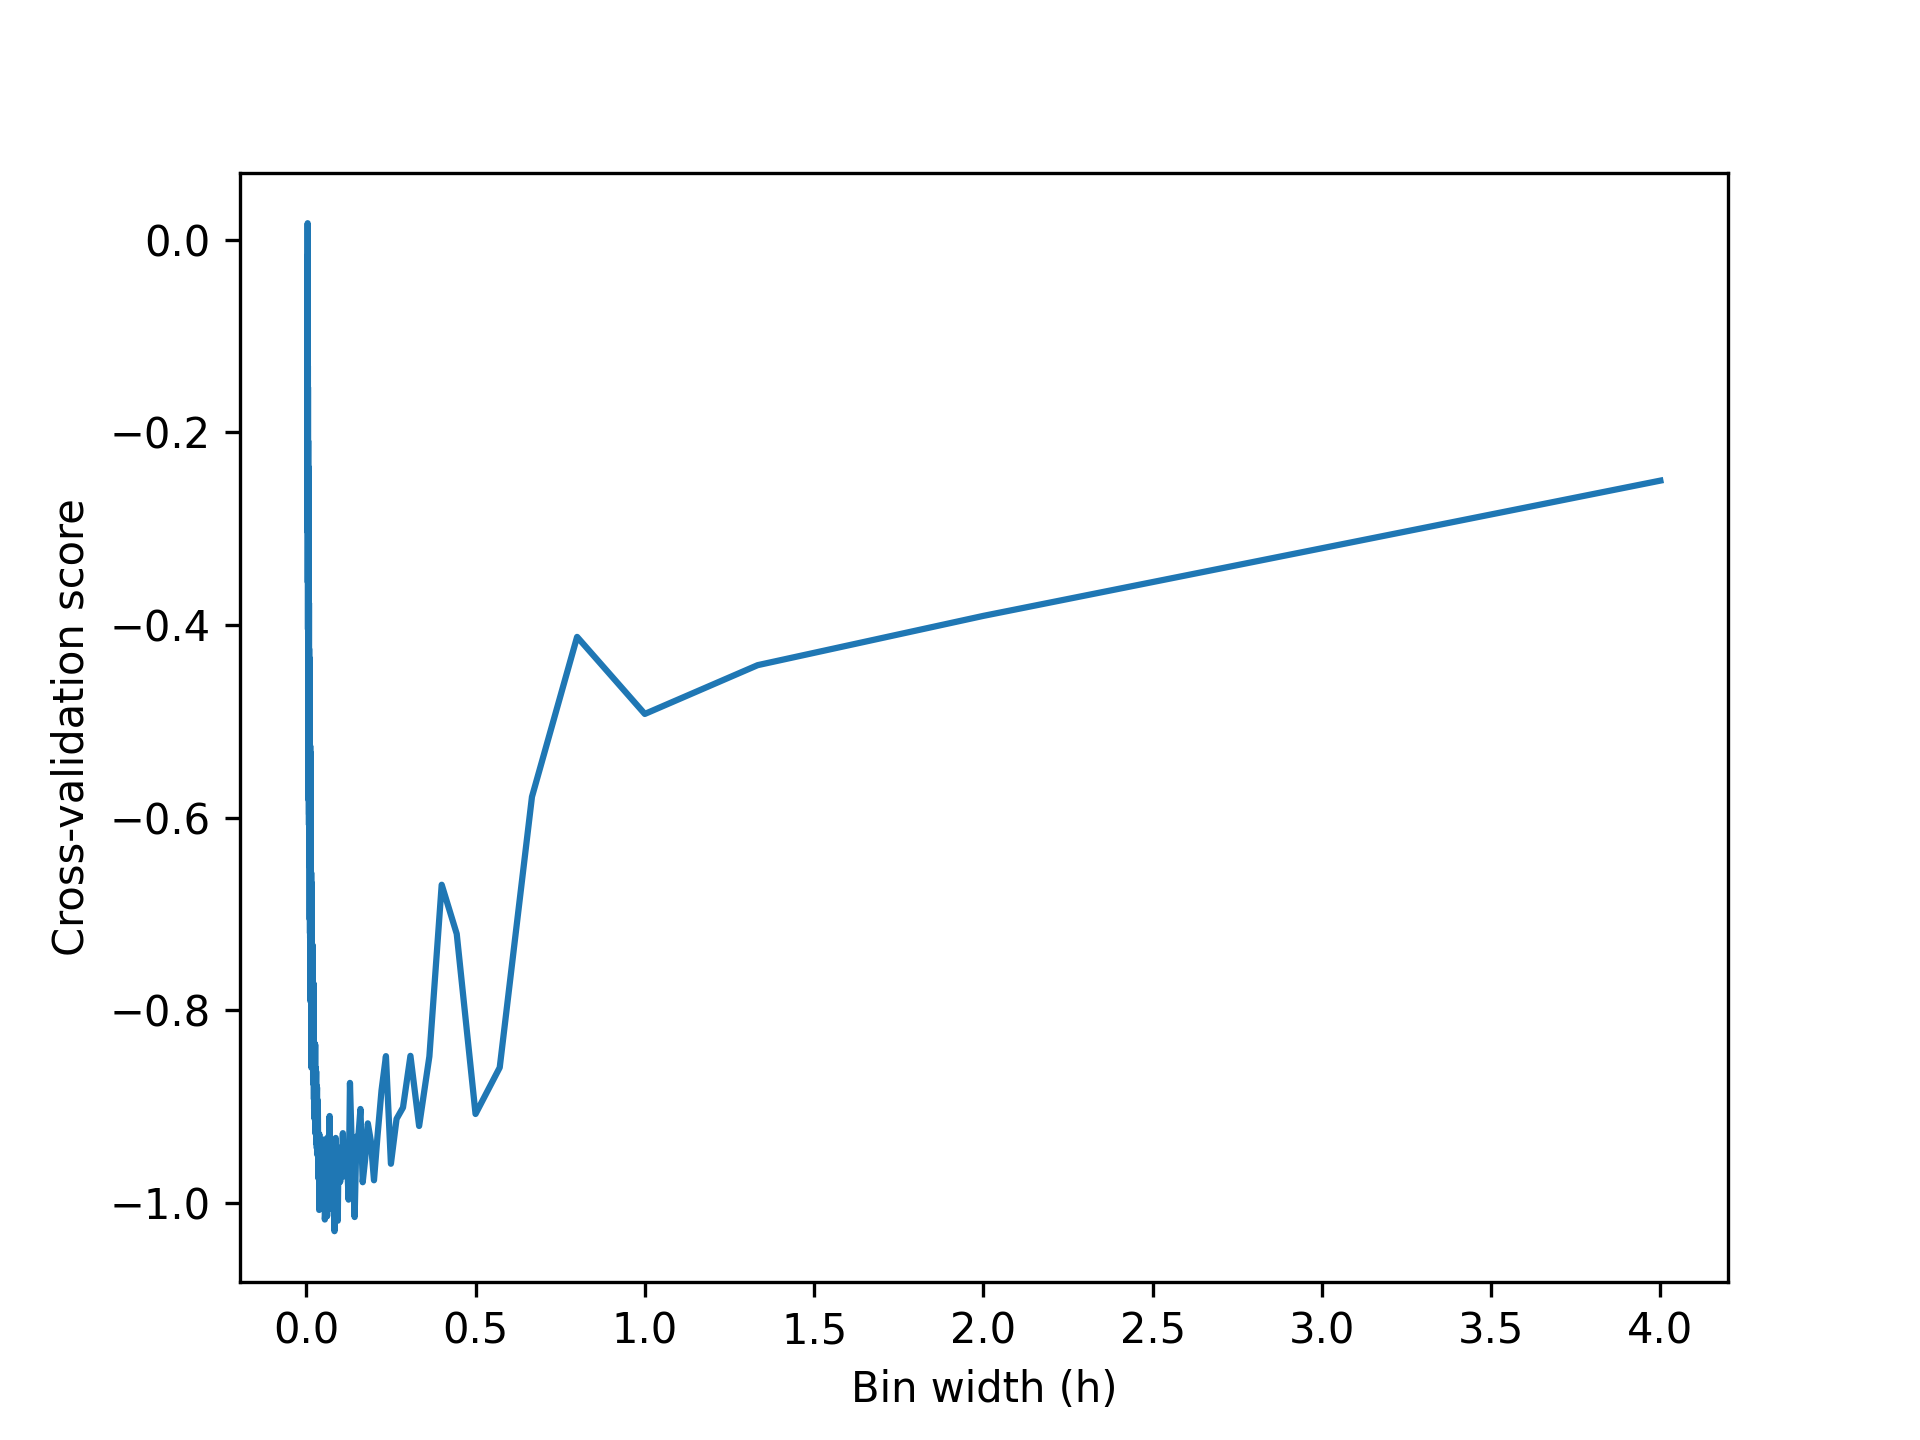
\includegraphics[width=0.6\textwidth]{images/1/crossvalidation.png}
	\caption{Cross-validation score for 1-1000 bins}
\end{figure}

\subsubsection*{(d)}
Based on the cross-validation score, the optimal value of bin width is 0.083, and the optimal bin count is 48.

\subsubsection*{(e)}
\vspace{-30pt}
\begin{figure}[H]
	\centering
	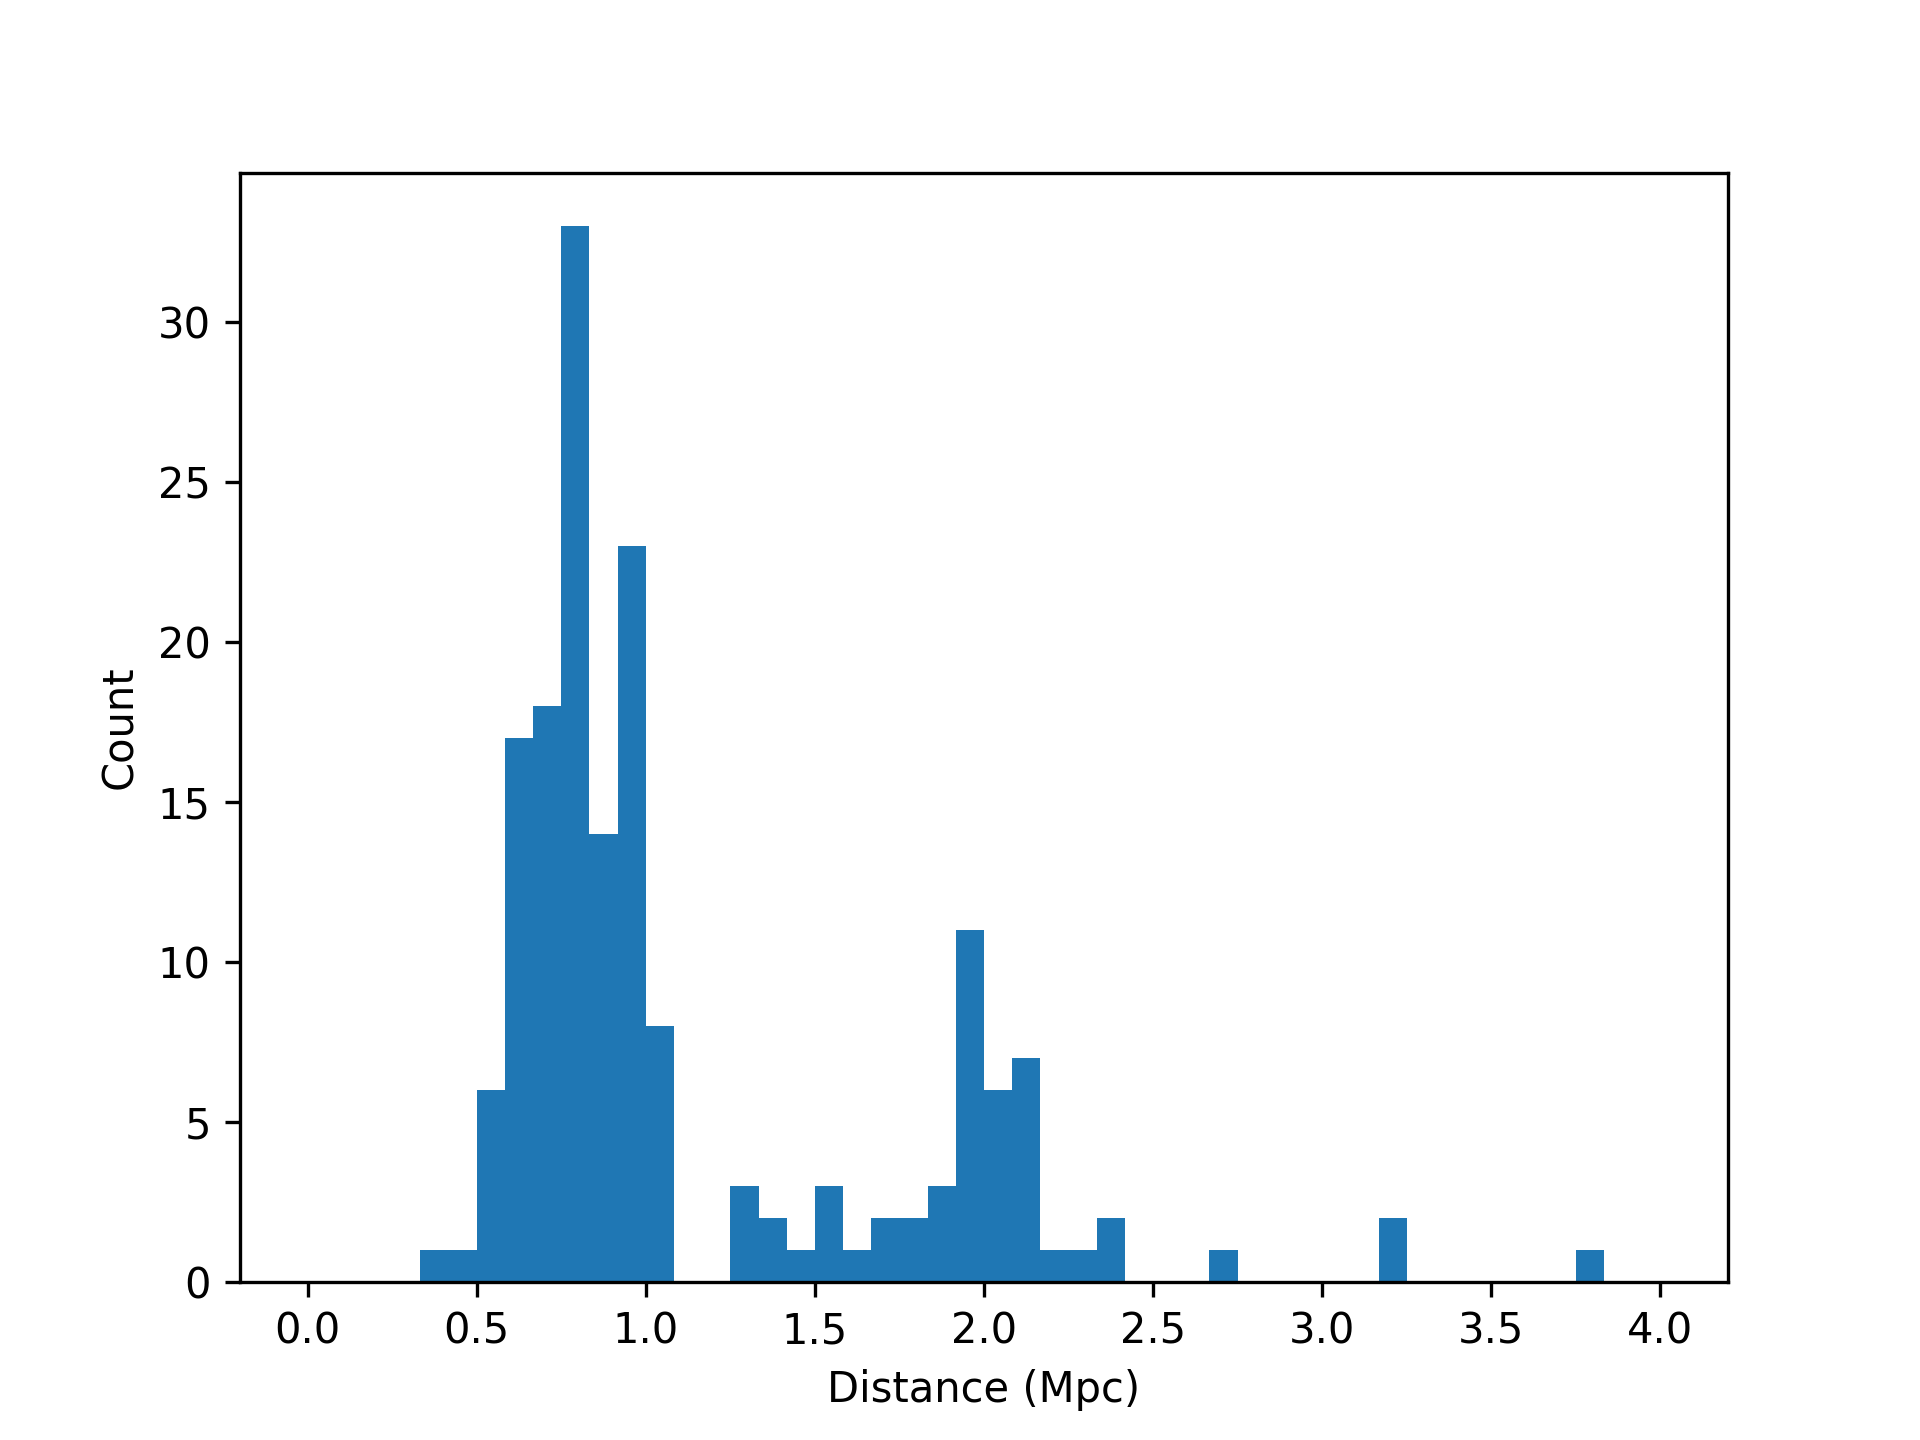
\includegraphics[width=0.6\textwidth]{images/1/optimalhistogram.png}
	\caption{Histogram with 48 bins}
\end{figure}

\subsubsection*{(f)}
Code is provided in \texttt{code/1.py}.
